\section{Affect of Data on our Techniques}
To get some more insight in to the behaviour of the indexing techniques that we applied, we performed further more analysis of the data. This gave us some further useful explanations.\\

\begin{figure}[ht!]	
\centering
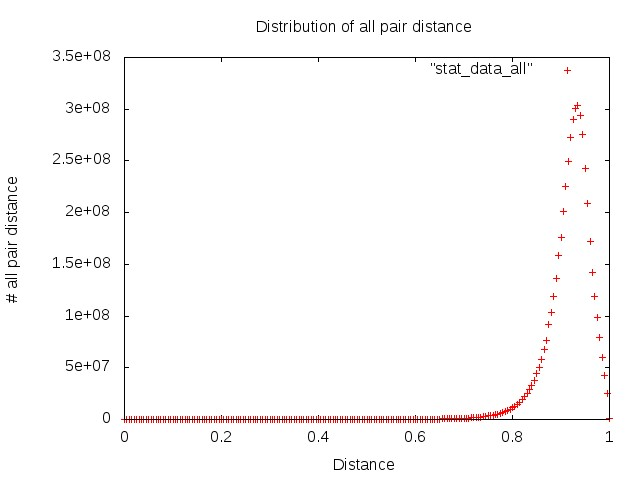
\includegraphics[width=0.35 \columnwidth]{img/all.jpg}
\caption{All pair distances}
\end{figure}
%\pagebreak
\begin{figure}[ht!]	
\centering
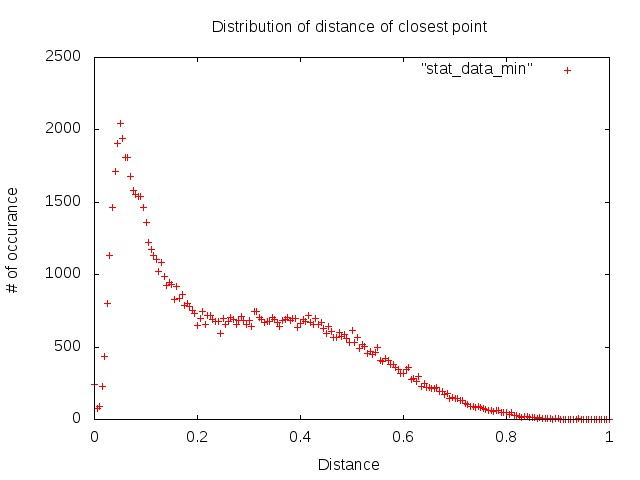
\includegraphics[width=0.35 \columnwidth]{img/min.jpg}
\caption{Distance of the closest point}
\end{figure}

\begin{figure}[ht!]	
\centering
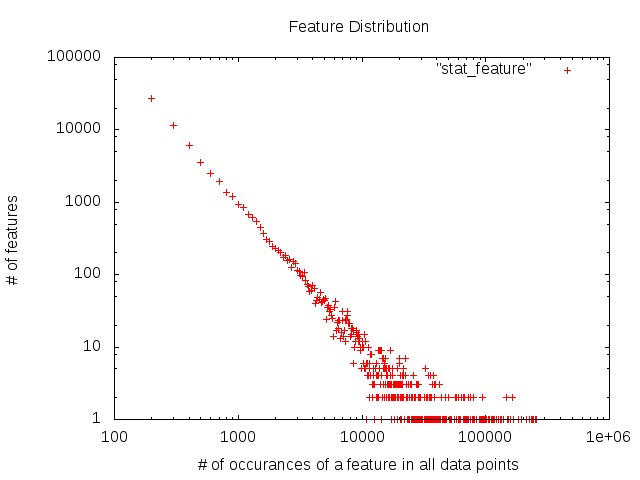
\includegraphics[width=0.35 \columnwidth]{img/feature.jpg}
\caption{Feature distribution}
\end{figure}

What we can observe from the data are the following:
\begin{enumerate}

\item {The being in high dimension, is very much spread out, and hence most of the points are equidistant from each other.}\\

\item {The closest point for most of the points is at distance much greater than 0.4. in fact only 0.007\% of the points have their 1-NN within a distance of 0.4.}\\

\item {the distribution of features among the data points seem to follow a power law distribution (though we have not tried to regress the plot to a function) i.e., even though we have many features only a hand full of them are repeated in most of the points.}\\

\end{enumerate}

These observations have many profound impact on our algorithms.
\begin{enumerate}

\item[A.] {One of the most time consuming operations in our algorithms has been the recurring theme of finding the set of maximally separated points, which we called as pivots. It takes hours for the algorithm to converge. Given the distribution of all pairs distance, we cannot hope to improve it further, but we can propose an heuristic streaming algorithm to handle it efficiently.\\ 
	We can maintain a list of most frequently occurring farthest points. These points are not necessarily the points farthest from each other, but the points which are most frequent in the list farthest points, for each point. This is motivated from the frequency counting problem from streaming as shown in \citet*{metwally2005efficient}.}\\

\item[B.] {We observed that the inverted index we proposed could not be easily generalised  to range queries. This can be further observed from the fact that how skewed the data distribution is.\\ 
	Given that only 0.007\% of the 1-nn points have distance less that 0.4, we can never achieve a efficient pruning. And in addition the distribution of heavy-hitters (features with occurrence more that 50000) is also very high, We have on an average 44 heavy hitters in a data point. Hence, in the worst case, we will be forced to explore all the points.} \\

\item[C.] {The success of any embedding technique, especially Lipschitz, depends on the ability of the reference set to be representative of the entire data. in our case, given that the entire data is very widely spread, the number of reference set required to well represent the data, becomes very large. This is the reason why Lipschitz did not give the desired results.}
\end{enumerate}
